%%%%%%%%%%%%%%%%%%%%%%%%%%%%%%%%%%%%%%%%%%%%%%%%%%%%%%%%%%%%%%%%%%%%%%
%%	Name: "Signal analysis template"
%%	File name: signalanalysis_template_main
%%	Version: 1.5
%%
%%	Compiler: XeLaTeX
%%
%%%%%%%%%%%%%%%%%%%%%%%%%%%%%%%%%%%%%%%%%%%%%%%%%%%%%%%%%%%%%%%%%%%%%%

\documentclass[conference,compsoc,onecolumn]{IEEEtran}

% *** LANGUAGE UTILITY PACKAGES ***
\usepackage[utf8]{inputenc} % Required for including letters with accents
\usepackage[spanish]{babel}

% *** USED PACKAGES ***
% *** MISC UTILITY PACKAGES ***
\usepackage{comment}			% Agregar comentarios
\usepackage{lipsum}				% Inserts dummy text
\usepackage{blindtext}
\usepackage{listings}					% Coding
\usepackage{verbatim}				% Verbatim
\usepackage[final]{pdfpages}
\usepackage{booktabs,dcolumn}
\usepackage{pdflscape}
\usepackage{afterpage}
%\setlist[itemize]{noitemsep, nolistsep}
\usepackage[bookmarks=false]{hyperref}
\usepackage{tcolorbox}									% Coloured boxes, for LATEX examples and theorems, etc
\usepackage{color}
\usepackage{xcolor} % Required for specifying colors by name									% Color packages foreground and back­ground color man­age­men
% *** CITATION PACKAGES ***
\usepackage{cite}
% *** GRAPHICS RELATED PACKAGES ***
\usepackage{graphicx}
\usepackage{caption}
\usepackage{pgfplots}
\usepackage{tikz}
\usetikzlibrary{shapes,arrows}
\usetikzlibrary{decorations.pathmorphing} % noisy shapes
\usetikzlibrary{fit}					% fitting shapes to coordinates
\usetikzlibrary{backgrounds}	% drawing the background after the foreground
\pgfplotsset{compat=1.13}
% *** MATH PACKAGES ***
\usepackage{amsmath}
\usepackage{mathtools}
\usepackage{amssymb}
\usepackage{amsfonts}
\usepackage{expl3}
\usepackage{bm}

% *** SPECIALIZED LIST PACKAGES ***
\usepackage{algorithmic}
\usepackage{listings}					% Coding
\usepackage[framed,numbered,autolinebreaks,useliterate]{mcode}
% *** ALIGNMENT PACKAGES ***
\usepackage{array}
% *** SUBFIGURE PACKAGES ***
%\ifCLASSOPTIONcompsoc
%\usepackage[caption=false,font=normalsize,labelfont=sf,textfont=sf]{subfig}
%\else
%\usepackage[caption=false,font=footnotesize]{subfig}
%\fi
% *** FLOAT PACKAGES ***
\usepackage{fixltx2e}
\usepackage{stfloats}
%\fnbelowfloat
%\usepackage{dblfloatfix}
% *** PDF, URL AND HYPERLINK PACKAGES ***
\usepackage{url}
\usepackage{everypage}


\usepackage{multirow} % In order to be able to insert rows spanning multiple lines
\usepackage{verbatim}
\usepackage[all]{xy}
\usepackage{listings}
\usepackage{subfigure}
\usepackage{multibib}
\usepackage{setspace} 
\usepackage{algorithm}			    	  % To insert nice algorithms

% *** CARPETA DONDE SE GUARDARAN LAS IMAGENES ***
\graphicspath{{img/}}

% *** NUEVOS COMANDOS Y CONFIGURACIONES VARIAS ***
\interdisplaylinepenalty=2500
\newcommand{\Lpagenumber}{\ifdim\textwidth=\linewidth\else\bgroup
	\dimendef\margin=0
	\ifodd\value{page}\margin=\oddsidemargin
	\else\margin=\evensidemargin
	\fi
	\raisebox{\dimexpr -\topmargin-\headheight-\headsep-0.5\linewidth}[0pt][0pt]{%
		\rlap{\hspace{\dimexpr \margin+\textheight+\footskip}%
			\llap{\rotatebox{90}{\thepage}}}}%
	\egroup\fi}
\newcommand{\linebreakand}{%
  \end{@IEEEauthorhalign}
  \hfill\mbox{}\par
  \mbox{}\hfill\begin{@IEEEauthorhalign}
}

\AddEverypageHook{\Lpagenumber}%

\newcommand{\newtxt}[1]{\textcolor{black}{#1}}
\renewcommand\IEEEkeywordsname{Palabras cláve:}
\newcommand{\mx}[1]{\mathbf{\bm{#1}}} % Matrix command
\newcommand{\vc}[1]{\mathbf{\bm{#1}}} % Vector command

%% Separación de palabras
\hyphenation{op-tical net-works semi-conduc-tor HHMMSS}

\begin{document}

% *** TITLES AND NAMES ***
% title of the document
\title{Seguimiento de datos COVID-19 en Colombia}
% author names and affiliations
\author{
    \IEEEauthorblockN{Santiago Gutiérrez Orjuela}
    \IEEEauthorblockA{Escuela de Ciencias exactas e Ingeniería\\
        Universidad Sergio Arboleda - Bogotá, Colombia\\
        santiago.gutierrez02@correo.usa.edu.co}
    \and
    \IEEEauthorblockN{Valeria Bermúdez Galván}
    \IEEEauthorblockA{Escuela de Ciencias exactas e Ingeniería\\
        Universidad Sergio Arboleda - Bogotá, Colombia\\
        valeria.bermudez01@correo.usa.edu.co}
    \linebreakand
    \IEEEauthorblockN{Juan Sebastián Bueno Ramírez}
    \IEEEauthorblockA{Escuela de Ciencias exactas e Ingeniería\\
        Universidad Sergio Arboleda - Bogotá, Colombia\\
        juan.bueno01@correo.usa.edu.co}}

% *** MAKE TITLE ***
\maketitle
\IEEEoverridecommandlockouts
\IEEEpeerreviewmaketitle

\begin{abstract}
En el presente documento se aplica la extracción de datos en internet sobre el coronavirus en Colombia para de forma selectiva presentarlos mediante diferentes gráficos. Se realiza código en Python, haciendo uso de web scraping para extraer los datos del Covid-19, se manipularán y visualizarán empleando librerias tales como pandas y matplotlib. 
\end{abstract}

\begin{IEEEkeywords}
    Python, web scraping, datos, Covid-19.
\end{IEEEkeywords}

\section{Marco teórico}
\label{sec:introduction}
El \textbf{coronavirus} es una familia de virus que causa infecciones respiratorias que pueden ir desde el resfriado común hasta el síndrome repiratorio agudo severo. El coronavirus que se ha descubierto más recientemente causa la enfermedad por coronavirus \textbf{COVID-19}, del cuál los síntomas más habituales son fiebre, tos seca y cansancio. Para el estudio del impacto que ha causado esta enfermedad causada por el virus, se representará en gráficos la información que se tiene de los casos confirmados en el país de Colombia.

Los \textit{datos abiertos} del gobierno de Colombia nos permitió acceder a la información asociada a los casos positivos de COVID-19, haciendo uso de web scraping en Python con \textb{sodapy} que es una biblioteca que funciona como cliente en la \textit{Socrata Open Data API}, estableciendo así conexión con la página del gobierno y obteniendo los datos necesarios, guardándolos como formato csv, estos se guardan en un dataframe con el uso de \textbf{Pandas}, el cual es una biblioteca que facilita la manipulación de estructuras de datos y nos brinda herramientas para el análisis de datos \cite{Pandas}. Para la visualización de los datos, se hace uso de \textbf{Matplotlib}, esta biblioteca nos permite hacer gráficas en 2D in Python, originalmente fue un emulador de los comandos de gráficos de MATLAB.

\section{Resultados}
\label{sec:results}
Para el uso de \textit{sodapy} para acceder a \texttt{Socrata}, escribimos las siguientes líneas, obteniendo así las $100000$ primeras filas de la tabla
\begin{lstlisting}[language=python]
from sodapy import Socrata
import pandas as pd
from datetime import datetime
import matplotlib.pyplot as plt
from collections import Counter


client = Socrata("www.datos.gov.co", None) #Se determina la dirección de la cual se extraerán los datos
results = client.get("gt2j-8ykr", limit=100000) #Se obtienen los datos y se establece un límite

# Convertir a dataframe de pandas
results_df = pd.DataFrame.from_records(results)
\end{lstlisting}

Con el fin de usar buenas prácticas, se llenan los espacios en blanco con el campo "No definido".

\begin{lstlisting}[language=python]
df=results_df
df=df.fillna('No Definido') #Se llenan los datos vacíos
tupla = (("T00:00:00.000", ""),("-", "/"))
for c in df.index:
    for a, b in tupla:
        df['fecha_de_notificaci_n'][c] = df['fecha_de_notificaci_n'][c].replace(a, b)
        df['fis'][c] = df['fis'][c].replace(a, b)
        df['fecha_diagnostico'][c] = df['fecha_diagnostico'][c].replace(a, b)
        df['fecha_recuperado'][c] = df['fecha_recuperado'][c].replace(a, b)
        df['fecha_reporte_web'][c] = df['fecha_reporte_web'][c].replace(a, b)
        df['fecha_de_muerte'][c] = df['fecha_de_muerte'][c].replace(a, b)
df.head()
\end{lstlisting}

A continuación , se muestra el código usado para preparar la data y crear las gráficas necesarias.
\begin{lstlisting}[language=python]
#Se convierten los datos de string a datatime object
for c in df.index:
    if(df['fecha_de_notificaci_n'][c]!='No Definido'):
        df['fecha_de_notificaci_n'][c]=datetime.strptime(df['fecha_de_notificaci_n'][c], '%Y/%m/%d')
    if(df['fis'][c]!='No Definido'):
        df['fis'][c]=datetime.strptime(df['fis'][c], '%Y/%m/%d')
    if(df['fecha_diagnostico'][c]!='No Definido'):
        df['fecha_diagnostico'][c]=datetime.strptime(df['fecha_diagnostico'][c], '%Y/%m/%d')
    if(df['fecha_recuperado'][c]!='No Definido'):
        df['fecha_recuperado'][c]=datetime.strptime(df['fecha_recuperado'][c], '%Y/%m/%d')
    if(df['fecha_reporte_web'][c]!='No Definido'):
        df['fecha_reporte_web'][c]=datetime.strptime(df['fecha_reporte_web'][c], '%Y/%m/%d')
    if(df['fecha_de_muerte'][c]!='No Definido'):
        df['fecha_de_muerte'][c]=datetime.strptime(df['fecha_de_muerte'][c], '%Y/%m/%d')
        
x=[] 
x=df['fecha_de_notificaci_n'] #Se llena con la fecha de notificación 
c=Counter(x) #Se cuentan los datos según la fecha de notificación
df1 = pd.DataFrame() #Se crea una nueva referencia del DataFrame
df1['Fecha']=c.keys() #Se extraen los elementos únicos
df1['No. Casos']=c.values() #Se extrae la frecuencia de cada elemento único
df1=df1.sort_values(by='Fecha') #Se ordenan según la fecha 

x = df1['Fecha'] #Se asignan los valores al eje x
y = df1['No. Casos'] #Se asignan los valores al eje y
plt.plot(x,y) #Se grafica
plt.title('Número de Casos')
plt.xlabel('Fecha')
plt.ylabel('No. Casos')
plt.savefig('Número de Casos.png') #Se guarda la imagen

import matplotlib
import numpy as np

y=[]
y=df['ciudad_de_ubicaci_n'] #Se llena con la ciudad
d=Counter(y) #Se cuentan los datos según la ciudad 
df2 = pd.DataFrame()
df2['Ciudad']=d.keys() #Se extraen los elementos únicos
df2['No. Casos']=d.values() #Se extrae la frecuencia de cada elemento único
df2=df2.sort_values(by='No. Casos',ascending=False) #Se ordena según el número de casos 

plt.figure(figsize=(10,7)) #Se establece el tamaño de la figura
#Colocamos etiquetas a los ejes
plt.xlabel("Ciudades")                       
plt.ylabel("Número de Casos") 

#Creamos la grafica de barras utilizando 'Ciudad' como eje X y 'Número de casos' como eje y.
x = df2['Ciudad'].iloc[0:6]
y = df2['No. Casos'].iloc[0:6]
plt.title("Ciudades con mayor número de Contagiados")
plt.bar(x, y)
#Finalmente mostramos la grafica con el metodo show()
plt.savefig('Ciudades.png')
plt.show()

tipo=[]
tipo=df['tipo']
#Se cuentan los casos según el tipo de contagio
e=Counter(tipo)
df3 = pd.DataFrame()
#Se establecen los elementos y la frecuencia de cada uno
df3['Tipo']=e.keys()
df3['No. Casos']=e.values()
#Se ordenan
df3=df3.sort_values(by='No. Casos',ascending=False)

#Se grafica el diagrama de torta 
plt.pie(df3['No. Casos'], labels=df3['Tipo'], autopct="%0.1f %%")
plt.axis("equal")
plt.title("Casos Totales por tipo de contagio")
plt.savefig('TipoContagio.png')
#Se muestra la grafica
plt.show()

estado=[]
estado=df['estado']
#Se cuentan los casos según el estado de los pacientes 
f=Counter(estado)
df4 = pd.DataFrame()
#Se establecen los elementos y la frecuencia de cada uno
df4['Estado']=f.keys()
df4['No. Casos']=f.values()
df4=df4.sort_values(by='No. Casos',ascending=False)

#Se grafica el diagrama de torta 
plt.pie(df4['No. Casos'], labels=df4['Estado'], autopct="%0.1f %%")
plt.axis("equal")
plt.title("Estado de los pacientes")
plt.legend()
plt.savefig('EstadoPacientes.png')
plt.show()

pais=[]
pais=df['pa_s_de_procedencia']
#Se cuentan los casos según el país de procedencia 
h=Counter(pais)
df6 = pd.DataFrame()
#Se establecen los elementos y la frecuencia de cada uno
df6['Pais de Procedencia']=h.keys()
df6['No. Casos']=h.values()
df6=df6.sort_values(by='No. Casos',ascending=False)
#Se hace una copia del data frame 
df6copy = df6.iloc[1:8].copy()
#Se organizan según el número de casos 
df6copy=df6copy.sort_values(by='No. Casos')

plt.figure(figsize=(9,7))
#Creamos la grafica pasando los valores en el eje X, Y, donde X = No de Casos y Y = País de Procedencia
x = df6copy['Pais de Procedencia']
y = df6copy['No. Casos']
plt.barh(x, y, align='center', alpha=0.5)
#añadimos una etiqueta en el eje X
plt.xlabel('Número de Casos')
plt.title('País de Procedencia')
plt.savefig('Pais.png')
plt.show()

muertes=[]
muertes=df['fecha_de_muerte']
#Se cuentan los casos según la fecha de muerte
g=Counter(muertes)
df5 = pd.DataFrame()
#Se establecen los elementos y la frecuencia de cada uno
df5['Muertes']=g.keys()
df5['No. Casos']=g.values()
df5=df5.sort_values(by='No. Casos',ascending=False)
#Se hace una copia del data frame 
copiamuertes=df5.iloc[1::].copy()

#Se organiza según el número de muertes 
copiamuertes=copiamuertes.sort_values(by='Muertes')
x = copiamuertes['Muertes']
y = copiamuertes['No. Casos']
#Se grafica
plt.plot(x,y)
plt.title('Fallecimientos  ')
plt.xlabel('Fecha')
plt.ylabel('Muertes')
#Se guarda la gráfica como .png
plt.savefig('Fallecimientos.png')
\end{lstlisting}

Mediante los datos extraídos de la página del Ministerio de Colombia, se realizó la gráfica de crecimiento de los casos desde el mes de marzo hasta el mes de julio , correspondiente al número de datos extraídos. Evidenciando el aumento de los casos a lo largo de los meses.
\begin{figure}[H]
    \centering
    \includegraphics{Número de Casos.png}
    \caption{Número de casos positivos por meses en Colombia}
    \label{fig:NumeroCasos}
\end{figure}

En la siguiente gráfica, se muestran las ciudades con mayor número de contagios dando cuenta que Bogotá DC es la que posee mayor número de contagios.
\begin{figure}[H]
    \centering
    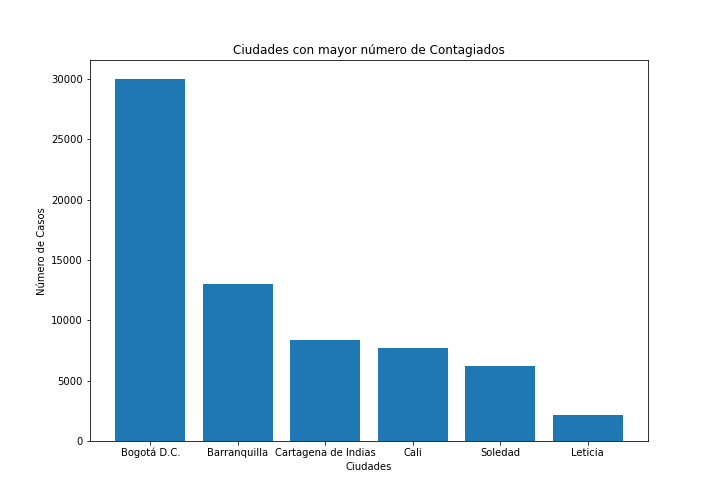
\includegraphics[keepaspectratio,width=0.8\textwidth]{Ciudades.png}
    \caption{Número de contagios por ciudad en Colombia}
    \label{fig:CasosCiudad}
\end{figure}

Luego, se realizó una gráfica de tortas con el fin de observar el estado de los pacientes según sus sintomas, ya sea leve, asintomatico, moderado, fallecido, grave, N/A permitiendo observar que el 83\% de los pacientes poseen sintomatología leve.
\begin{figure}[H]
    \centering
    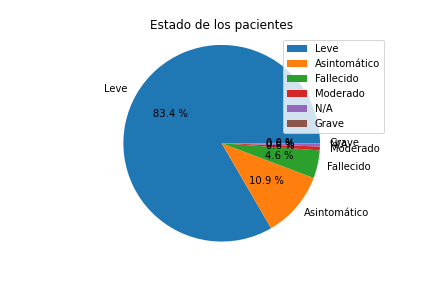
\includegraphics[keepaspectratio,width=0.6\textwidth]{EstadoPacientes.png}
    \caption{Estado de los pacientes de COVID-19 en Colombia}
    \label{fig:EstadoPacientes}
\end{figure}

También, se realizó un gráfico de tortas para saber qué tipos de contagios poseen las personas aunque con el aumento exponencial de casos la mayoría de casos han quedado en estudio.
\begin{figure}[H]
    \centering
    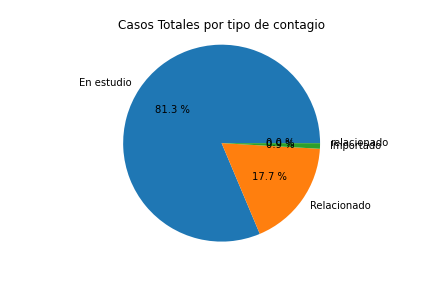
\includegraphics[keepaspectratio,width=0.8\textwidth]{TipoContagio.png}
    \caption{Tipo de contagio en pacientes colombianos}
    \label{fig:TipoContagio}
\end{figure}

Posteriormente, se graficó el número de fallecidos por mes donde se puede evidenciar que el mes con mayor cantidad de muertos hasta el día de hoy es Julio.
\begin{figure}[H]
    \centering
    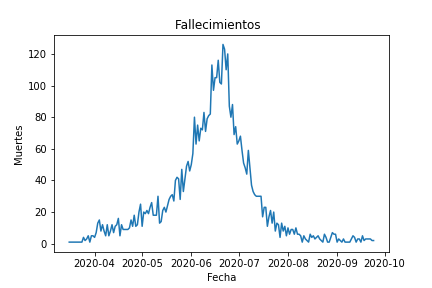
\includegraphics[keepaspectratio,width=0.8\textwidth]{Fallecimientos.png}
    \caption{Número de fallecidos por mes en Colombia}
    \label{fig:FallecidosMes}
\end{figure}

Por último, mediante un gráfico de barras se mostró que la mayoría de casos importados provienen de los países España y Estados Unidos, quienes ya tuvieron su pico de la pandemia.
\begin{figure}[H]
    \centering
    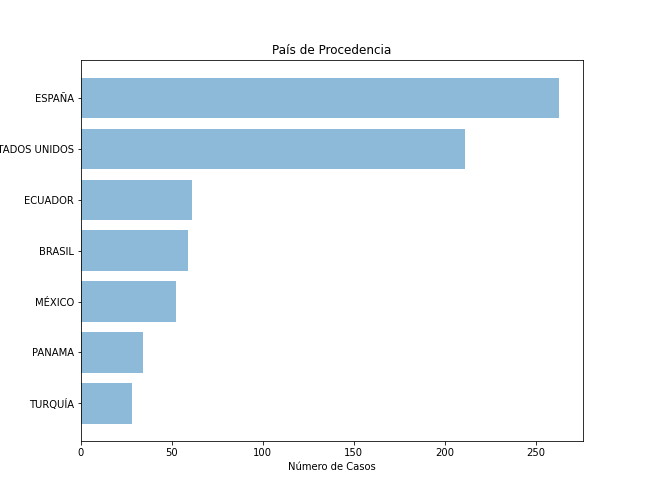
\includegraphics[keepaspectratio,width=0.8\textwidth]{Pais.png}
    \caption{País de procedencia de los pacientes importados}
    \label{fig:PaisProcedencia}
\end{figure}

\section{Conclusiones}
\label{sec:conclusions}
Se identifica que Pandas y Matplotlib nos facilita el manejo de los datos y su visualización.

Se evidencia que el número de contagios crece exponencialmente, tal como se ve en la figura \ref{fig:NumeroCasos}.

Más del 80\% de los contagios no se sabe de dónde vienen, siguen en estudio, esto debido al crecimiento exponencial de casos no permitiendo determinar la proveniencia de la mayoría de contagios.

Bogotá es la ciudad con más contagios debido a ser la que tiene más habitantes y además donde llegan los vuelos internacionales.

\nocite{*}
\bibliographystyle{IEEEtran}
\label{sec:biblio}
\bibliography{bib/biblio} 





%\pagestyle{empty}
\end{document}


